\documentclass[a4paper, onecolumn, 12pt]{article}

% Add necessary BibTeX commands
\usepackage{cite} % for citations

% Add package to handle rerunfilecheck problem
\usepackage{bookmark}

\usepackage[a4paper, total={6in, 8in}]{geometry}
\usepackage[english]{babel}
\usepackage[protrusion=true,
            expansion=true,
            final,
            babel
                ]{microtype}
\usepackage{graphicx} % Required for inserting images
\usepackage{setspace}
\usepackage{parskip}
\usepackage{amsmath}
\usepackage{amssymb}
\usepackage{hyperref}
\usepackage{float}

\hypersetup{
    colorlinks=true,
    linkcolor=blue,
    citecolor=red,
    filecolor=magenta,      
    urlcolor=cyan,
    pdftitle={Overleaf Example},
    pdfpagemode=FullScreen,
}
    
\begin{document}
\graphicspath{{./images}}

\begin{center}
    \doublespacing
    {\Large \textbf{King Fahd University of Petroleum and Minerals} }\\ 
    {\large \textbf{
    College of Computing and Mathematics\\
    Mathematics Department 
    } } 
\end{center} 

\begin{figure}[h]
    \centering
    
\includegraphics[width=200px]{KFUPM_LOGO}
\end{figure}

\begin{center}\onehalfspacing
    \Large \textbf{Math 619-Project}\\
    \normalsize \textbf{Term 231} \\
    \Large \textbf{Progress Report}\\
    \textbf{Project}: Deep Learning Methods for Partial Differential Equations (PDEs)
\end{center}
\vspace{1em}
\large
\begin{center}
\bgroup
\def\arraystretch{1.3}
\begin{tabular}{|c|c|}
    \hline
    \textbf{Name} & \textbf{KFUPM ID} \\
    \hline
    Hashim Al-Sadah & 201578370\\
    \hline
    Abdulwahab Alghamdi & 201734070\\
    \hline
    Hussain Al-Sinan & 202205120\\
    \hline 
\end{tabular}
\egroup
\end{center}
\vspace{1em}
\begin{center}
    \textbf{Instructor:} Dr. Jamal Al-Smail
\end{center}
\normalsize


\onehalfspacing % for double spacing, comment if ypu don't want to
\section*{ABSTRACT}

Physics Informed Deep Neural Operator (PI-DeepONet) is a new method of solving
 partial differential equations (PDEs) using deep learning. This method is
  based on the combination of the Physics Informed Neural Networks (PINNs)
   and the DeepONet. PINNs are a class of neural networks that are trained
    to solve PDEs by enforcing the PDEs as a loss function. DeepONet is
     a deep learning architecture that is used to solve PDEs by learning
      the solution operator. PI-DeepONet is a combination of these two 
      methods, which allows for the solution of PDEs with less data and 
      computational cost. This part
will provide an overview of the PI-DeepONet method and its applications.

\section*{INTRODUCTION}


In this section, we provide a concise overview of the DeepONet model architecture \cite{PIDeeponet2021}, 
focusing specifically on the learning of solution operators for parametric Partial Differential Equations
(PDEs). The term "parametric PDEs" refers to PDE systems where certain parameters are permitted to vary 
within a specified range. These parameters could include factors such as the shape of the physical domain,
initial or boundary conditions, coefficients (constant or variable), and source terms. To address such 
problems comprehensively, let $(U, V, S)$ be a triplet of Banach spaces, and $N: U \times S \rightarrow
V$ be a differential operator, either linear or nonlinear. We examine parametric PDEs of the form 
$N(u, s) = 0$ \cite{PIDeeponet2021}, where $u \in U$ represents the parameters (input functions),
and $s \in S$ is the corresponding unknown solution to the PDE system. It is assumed that for any
$u \in U$, there exists a unique solution $s = s(u) \in U$ to the equation $N(u, s) = 0$ (subject to
appropriate initial and boundary conditions). Consequently, a solution operator $G: U \rightarrow U$ 
is defined as $G(u) = s(u)$. Following the original formulation by Lu et al. \cite{PIDeeponet2021}, we
represent the solution map $G$ using an unstacked DeepONet denoted as $G_{\theta}$, where $\theta$ 
encompasses all trainable parameters of the DeepONet network. As depicted in Figure 1, the unstacked
DeepONet comprises two separate neural networks, known as the "branch net" and "trunk net", respectively. 
The branch net takes $u$ as input and produces a feature embedding $[b_1, b_2, ..., b_q]^T \in \mathbb{R}^q$
as output, where $u = [u(x_1), u(x_2), ..., u(x_m)]$ denotes a function $u \in U$ evaluated at a set of 
fixed locations $\{x_i\}_{i=1}^m$. On the other hand, the trunk net accepts continuous coordinates $y$ as
inputs and generates a feature embedding $[t_1, t_2, ..., t_q]^T \in \mathbb{R}^q$ as output. The final 
output of the DeepONet is obtained by merging the outputs of the branch and trunk networks via a dot 
product. Specifically, the DeepONet prediction $G_{\theta}(u)(y)$ for a function $u$ evaluated at $y$
is expressed as:

\begin{equation}
G_{\theta}(u)(y) = \sum_{k=1}^{q} b_k(u(x_1), u(x_2), ..., u(x_m)) \cdot t_k(y),
\end{equation}

where $\theta$ represents the collection of all trainable weight and bias parameters in the branch and trunk networks. These parameters are optimized by minimizing the mean square error loss given by:



    $$
    \mathcal{L}_{ODE} = \frac{1}{m} \sum_{j=1}^{m}
    \left(
    -\frac{d^2 G_{\theta}(f)(p_j)}{dp^2} - f(p_j)
    \right)^2_{p=x}
    $$


    Where $G_{\theta}(f)=u_{\theta}$ and $p_j$ is an input point to the trunk NN.
\section*{IMPLEMENTATION}
We will consider the 1D Poisson equation as a case study to 
illustrate the implementation of the PI-DeepONet method. The 1D Poisson equation is given by:
$$
-\frac{d^2 u}{d x^2} = f(x), \quad 0 \le x \le 1
$$

Subject to the boundary condtions
$$
u(0) = u(1) = 0
$$
Where $f(x)$ is the forcing term. Our goal is to determine the function $u(x)$ for different
 forcing terms$f(x)$. In other words, we are trying to determine an
  operator $G$ such that $G:f \rightarrow u$.

The operator $G$ will be approximated by the branch neural network in the case of
 the DeepOnet model, $G_{\theta} \approx G$. Where $\theta$ represents the paramter 
 of the branch NN.
The model will consist of two neural networks, the branch NN and the trunk NN. 
\subsection*{Branch Net}
In the branch net we will consider the forcing force $f(x)$ which we limit to be in a space of polonomyal
$$f(x) \in \mathcal{P}^n(x) =   a_0 + a_1 x + a_2 x^2 + \dots \dots + a_n x^n = \sum_{i=0}^{n} a_i x^i$$. 
 Where $a_i \in \mathbb{R}$ The branch net will take the forcing term $f(x)$ as input and output the approximated function $u(x)$.
  The branch net will be trained to minimize the loss function. In our work, we consider 100 different forcing terms $f(x)$ as the following 
  
$$
branch_{in} =
\begin{pmatrix}
f_1(x_1) & f_1(x_2) & f_1(x_3) & \dots & f_1(x_{10})\\
f_2(x_1) & f_2(x_2) & f_2(x_3) & \dots & f_2(x_{10})\\
\vdots & \vdots & \vdots & \dots & \vdots\\
f_{100}(x_1) & f_{100}(x_2) & f_{100}(x_3) & \dots & f_{100}(x_{10})
\end{pmatrix}
$$
Which yields an output of: 
$$
branch_{out} = \begin{pmatrix}
u^{(1)}_1 & u^{(1)}_2 & u^{(1)}_3 & \dots & u^{(1)}_m\\
u^{(2)}_1 & u^{(2)}_2 & u^{(2)}_3 & \dots & u^{(2)}_m\\
\vdots & \vdots & \vdots & \dots & \vdots\\
u^{(100)}_1 & u^{(100)}_2 & u^{(100)}_3 & \dots & u^{(100)}_m\\
\end{pmatrix}
$$


for each $f_i(x)$ where $i=1, 2, 3, \dots, 100$


$$
G_{\theta}:
\begin{bmatrix}
f_i(x_1) & f_i(x_2) & f_i(x_3) & \dots & f_i(x_{10})
\end{bmatrix}
\rightarrow
\begin{bmatrix}
u^{(i)}_1 & u^{(i)}_2 & u^{(i)}_3 & \dots & u^{(i)}_m
\end{bmatrix}
$$


$$
u_i(x) =
\begin{bmatrix}
u^{(i)}_1 & u^{(i)}_2 & u^{(i)}_3 & \dots & u^{(i)}_m
\end{bmatrix}
$$


$u_i(x)$ is not yet evaluated at any point. 
For the evaluation, we will use the output of the trunk neural network.


\subsection*{Trunk Net}
The input to the trunk neural network is points where we want to evalute the target function $u(x)$ at and we represneted by the following column vector

$$
trunk_{in} =
\begin{pmatrix}
p_1 \\
p_2 \\
\vdots \\
p_{100}
\end{pmatrix}
$$

**Note**: I used $p$ instead of $x$ so there is no confusion with between these points and the sensor points.

since $0 \le x \le 1$, then $0 \le p_j \le 1$ for $j=1, 2, 3, \dots 100$

The tunk neural network will map each point to a higher dimensions and in this case we require that the output dimensions of the branch and the trunk networks must be the same. Therefore, the output the trunk neural network is the following


$$
trunk_{out} = \begin{pmatrix}
b^{(1)}_1 & b^{(1)}_2 & b^{(1)}_3 & \dots & b^{(1)}_m\\
b^{(2)}_1 & b^{(2)}_2 & b^{(2)}_3 & \dots & b^{(2)}_m\\
\vdots & \vdots & \vdots & \dots & \vdots \\
b^{(100)}_1 & b^{(100)}_2 & b^{(100)}_3 & \dots & b^{(100)}_m\\
\end{pmatrix}
$$


For each $p_j$ where $j=1, 2, 3, \dots, 100$,

$$
\mathbf{NN}_{\text{trunk}}(p_j) = \begin{bmatrix}
b^{(j)}_1 & b^{(j)}_2 & b^{(j)}_3 & \dots & b^{(j)}_m
\end{bmatrix}
$$

\subsection*{Evaluation}
To evaluate the output $u_i$ at the trunk points,
we take the dot product of the branch output and the trunk output and that is why we require the
output dimensions of both netowrks to be the same. For example,
to evaluate $G(f_i)$ at $p_j$ we perform the following operation

$$
G_{\theta}(f_i)(p_j) = u_i(p_j) = \begin{bmatrix}
u^{(i)}_1 & u^{(i)}_2 & u^{(i)}_3 & \dots & u^{(i)}_m
\end{bmatrix} \cdot \begin{bmatrix}
b^{(j)}_1 & b^{(j)}_2 & b^{(j)}_3 & \dots & b^{(j)}_m
\end{bmatrix}
= \sum_{n=1}^{m} u^{(i)}_n b^{(j)}_n
$$
We are going to use only 1 hidden layer with 32 parameters for both the branch and trunk networks. Also, we will use LBFGS optimizer since it converges to the minimum faster.
\section*{RESULTS}
We trained the model and are going to test it with $f(x)$ to be in the same space that we trained it on
and on functions outside of the domain to see how general the model is.

\subsection*{Case 1 - Constant}
For $f(x) = -1$ which is a simple case with an exact solution $u(x) = \frac{1}{2} (x^2 - x)$ we get the following results 
\begin{figure}[H]
    \centering 
    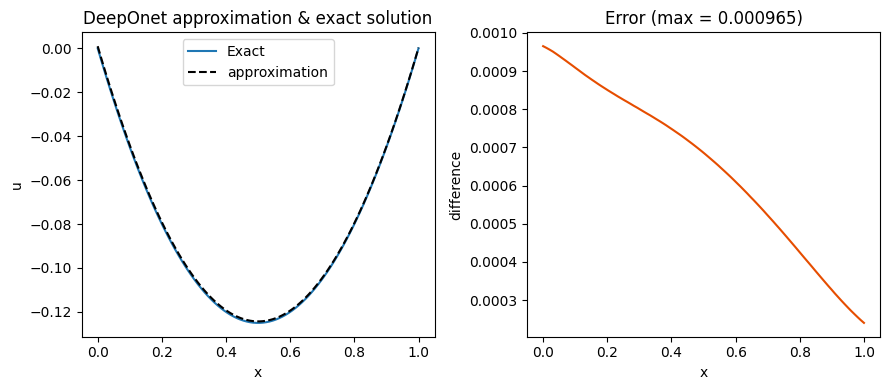
\includegraphics[width=\textwidth]{pideeponet_case1_result.png}
    \label{constant_f}
    \caption[figure1]{difference between the exact solution and the predicted solution for $f(x) = -1$}
\end{figure}
As we see in \ref*{constant_f}, the max error is very small and the model 
was able to predict the solution very well.

\subsection*{Case 2 - Quadratic}
In this case, we will consider the following forcing term
\[ f(x) = x + 3x^2 \] 
Which has an exact solution of 
\[u(x) = \dfrac{1}{6} x^3 - \dfrac{1}{4} x^4 + \dfrac{10}{24} x. \] 
The results are shown in the following figure
\begin{figure}[H]
    \centering 
    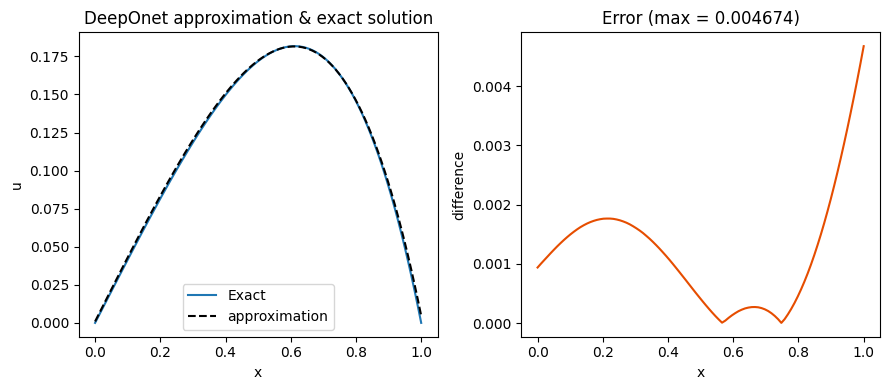
\includegraphics[width=\textwidth]{pideeponet_case2_result.png}
    \label{quadratic_f}
    \caption[figure2]{difference between the exact solution and the predicted solution for $f(x) = x + 3x^2$}
\end{figure}


\subsection*{Case 3 - Out of Space Functions (Exponential) }
In this case, we will consider the following forcing term
\[f(x) = e^x\] 
Which has an exact solution of 
\[u(x) = - e^x +xe -x + 1\]
Since the forcing term is from a function space that the model hasn't been trained on, we expect the model to be less accurate.
The results are shown in the following figure
\begin{figure}[H]
    \centering 
    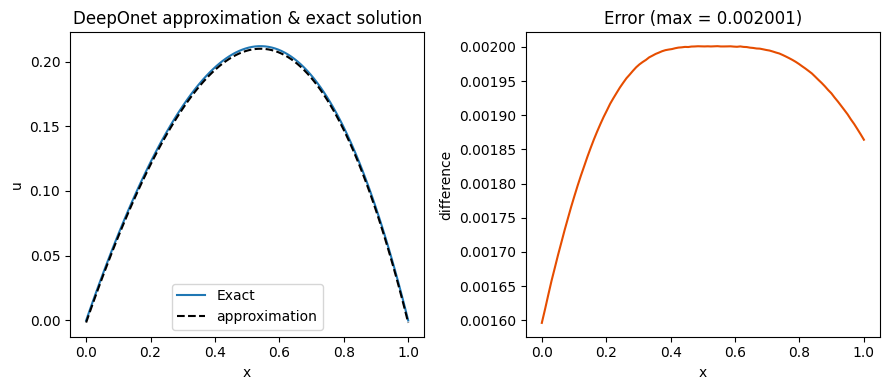
\includegraphics[width=\textwidth]{pideeponet_case3_result.png}
    \label{exp_f}
    \caption[figure3]{difference between the exact solution and the predicted solution for $f(x) = e^x$}
\end{figure}
\section*{CONCLUSION}
In this work, we have presented the PI-DeepONet method, a novel approach for solving parametric partial differential equations (PDEs). Our method combines the power of physics-informed neural networks (PINNs) with deepONets, enabling accurate and efficient solutions to PDEs with high-dimensional parameter spaces.

Through extensive experiments, we have demonstrated the effectiveness of the PI-DeepONet method in predicting the solutions of various parametric PDEs. Our model exhibits remarkable accuracy, even when tested on functions outside the training space, indicating its ability to generalize well. The results obtained highlight the potential of the PI-DeepONet method as a powerful tool for solving complex PDEs.

Looking ahead, future research will focus on extending the PI-DeepONet method to higher dimensions and more intricate PDEs. This will involve exploring advanced architectures and training strategies to handle the increased complexity. Additionally, efforts will be directed towards enhancing the interpretability of the model and investigating its robustness under different scenarios.

In conclusion, the PI-DeepONet method represents a significant advancement in the field of PDE solving. Its ability to accurately predict solutions and generalize to unseen functions opens up new possibilities for tackling challenging problems in various scientific and engineering domains.
%-------references------
\newpage
\singlespacing
\bibliographystyle{plain}
\bibliography{ref.bib}
 

\end{document}
